\chapter{The Frozen Spin (FS) method}\label{chpt1:top-level}

\section{General introduction}\label{chpt1:FS-introduction}

\subsection{The T-BMT equation}\label{sec:TBMT_introduction}
The Thomas-Bargmann-Michel-Telegdi equation describes the dynamics of a spin vector $\vec s$ in
a magnetic field $\vec B$ and electrostatic field $\vec E$. Its generalized version,
which includes the EDM effect, can be written as (in the beam rest frame):~\cite[p.~6]{Eremey:Thesis}
\begin{subequations}
  \begin{align}
    \ddt{\vec s} &= \vec s\times \bkt{\vec\W_{MDM} +\vec\W_{EDM}}, \label{eq:TBMT_main}
    \intertext{where the MDM and EDM angular velocities $\vec\W_{MDM}$ and $\vec\W_{EDM}$ }
    \vec\W_{MDM} &= \frac qm \bkt*{G\vec B - \bkt{G - \frac{1}{\gamma^2-1}}\frac{\vec E\times\vec\beta}{c}},\label{eq:TBMT_MDM} \\
    \vec\W_{EDM} &= \frac qm \frac\eta2 \bkt*{\frac{\vec E}c + \vec\beta\times \vec B}.\label{eq:TBMT_EDM}
  \end{align}
\end{subequations}
In the equations above, $m,~q,~G=(g-2)/2$ are respectively the particle mass, charge,
and anomalous magnetic moment; $\beta = \sfrac{v_0}{c}$, is its relative velocity factor;
$\gamma$ its Lorentz factor. The EDM factor $\eta$ is defined by $d = \eta\frac{q}{2mc}s$, where
$d$ is the particle EDM, $s$ its spin.

In the standard formalism it is usual to operate with the (rotational)
one-turn spin transfer matrix:~\cite[p.~4]{COSY:SpinTuneMapping}
\[
\bold{t}_R = \exp\bkt{-i\pi\nu_s\vec\sigma\cdot\bar n} = \cos\pi\nu_s - i (\vec\sigma\cdot\bar n)\sin\pi\nu_s,
\]

where $\nu_s = \sfrac{\W_s}{\W_{cyc}}$, the ratio of the partile's spin precession frequency
to its cyclotron frequency, is termed \emph{spin tune}, $\bar n$ defines the spin precession axis,
and is called the \emph{invariant spin aixs}.

\subsection{Frozen spin concept}
From equation~\eqref{eq:TBMT_MDM} one can see that, in the absence of an EDM,
the direction of a particle's spin vector can be fixed relative its momentum vector, i.e.
$\vec\W_{MDM}=\vec 0$; in other words, one can realize the Frozen Spin condition.

The advantage of working in the FS-regime:
according to equations~\cref{eq:TBMT_main,eq:TBMT_MDM,eq:TBMT_EDM}, the MDM and EDM
angular velocity vectors are orthogonal, meaning that htey add in squares in the net frequency,
and hence the frequency shift associated with the EDM becomes a second-order effect:~\cite[p.~5]{Mane:SpinWheel}
\[
\w \propto \sqrt{\W_{MDM}^2 + \W_{EDM}^2} \approx \W_{MDM} + \frac{\W_{EDM}^2}{2\W_{MDM}}.
\]
This circumstance significantly diminishes the experimental sensitivity.

However, by freezing the particle's spin in the horizontal plane, the only remaining
MDM angular velocity component is aligned with the EDM component, and hence adds to it
linearly, which greatly improves the sensitivity.

\subsection{Realization of the FS condition in a storage ring}\label{sec:FS_in_a_ring}
Storage rings can be classified into three groups:
\begin{enumerate}
	\item Purely magnetic (COSY, NICA, etc),
	\item purely electrostatic (Brookhaven AGS Analog Ring),
	\item combined.
\end{enumerate}

In view of equation~\eqref{eq:TBMT_MDM}, the FS condition cannot be realized in a purely magnetic ring.

For particles like the proton (whose $G>0$), a purely electrostatic ring can
be used in the FS methodological framework, if the beam has the so-called ``magic''
energy, defined as $\gamma_{mag} = \sqrt{(1+G)/G}$.

For particles whose $G<0$ (deuteron) this is impossible, and one is required to use a combined ring.
To realize the FS condition in a combined ring, a radial electric field is introduced~\cite{BNL:Deuteron2008}:
\begin{equation}\label{eq:FS_Er}
E_r = \frac{GB_yc\beta\gamma^2}{1-G\beta^2\gamma^2}.
\end{equation}


\section{FS-based methodologies}\label{chpt1:FS-methods}
In this section we first give two examples of foundational methods for searching for the EDM
in a storage ring, both of which are based on the FS idea;
then we generalize these methods to two mutually-exclusive categories;
we finish with the introduction of the 2D FS method.

We note, too, that apart from the FS method alternative approaches to the EDM measurement exist,
for example~\cite{COSY:SpinTuneMapping, COSY:Partially-Frozen-Spin}, in which the beam polarization
freely precesses about the vertical guiding field of the storage ring.

\newcommand{\wimp}{\w_{\avg{E_v}}}
\newcommand{\wsw}{\w_{SW}}
\newcommand{\wedm}{\w_{edm}}

\newcommand{\D}{\Delta}
\DeclareDocumentCommand{\g}{s}{\gamma\IfBooleanT{#1}{_{eff}}}

\subsection{BNL FS method}
The BNL FS method was proposed by the Storage Ring EDM Collaboration
of Brookhaven National Laboratory in 2008.~\cite{BNL:Deuteron2008}
It is a combined ring method. A longitudinally-polarized beam is
injected into the ring; with polarimetry measurements,
is spin precession is probed in the horizontal and vertical planes;
The EDM signal is the change in the vertical polarization component over time,
which is expressed by:~\cite[p.~8]{BNL:Deuteron2008}
\begin{equation}
  \Delta P_V = P\frac{\w_{edm}}{\W}\sin\bkt{\W t + \Theta_0},
\end{equation}
where $\W = \sqrt{\w_{edm}^2 + \w_a^2}$, $\w_a,~\w_{edm}$ are the angular velocities
generated by, repsectively, the magnetic and electric dipole moments.

By applyting a radial electric field $E_r$ (magnitude defined by equation~\eqref{eq:FS_Er}),
it is expected that the $\w_a$ component is attenuated by at least a factor of $10^9$; in view
of the smallness of the hypothesized value $\w_{edm}$, $\Delta P_V \approx P \w_{edm} t$,
and hence the maximum amplitude $\Delta P_V$ is amplified by $10^9$.

The expreriment is expected to reach a sensitivity level of $10^{-29}~e\cdot cm$ in $10^7$
seconds (6 months) of total measurement time. At this sensitivity level
cross section asymmetry $\varepsilon_{LR} \approx 5\cdot 10^{-6}$ for the smallest practical
calues of $\w_a$.~\cite[p.~18]{BNL:Deuteron2008} The latter circumstance creates a
serious problem for polarimetry.~\cite{Mane:SpinWheel} One way to solve it lies in applying
a radial magnetic field and measuring the net MDM+EDM spin precession frequency.
This is the basic idea of the so-called Spin Wheel method (also called Koop Wheel),
which is considered in the next section.

The only presently known first-order systematic effect of spin dynamics
is the presence of a non-zero average vertical electric field component $\avg{E_V}$.
In this case, spin precesses about the radial axis at a rate~\cite[p.~11]{BNL:Deuteron2008}
\[
\w_{syst} \approx \frac{\mu\avg{E_V}}{\beta c\gamma^2}.
\]
Two circumstances are important here:
\begin{itemize}
\item the presence of $\avg{E_V}\neq 0$ is due to lattice element alignment error;
\item This systematic effect changes sign when the beam is injected in the opposite direction.
\end{itemize}
The latter is why the clockwise/anti-clockwise beam injection pattern is used in the 2D FS method.
Even though $\w_{syst}$ changes sign when the beam circuation direction is reversed (and hence is
susceptible to control), this methodology does not account for its \emph{magnitude}.
In section~\ref{chpt3:imperfections} (numerically, in~\ref{chpt3:imperfections:magnitude}), 
show that at a realistic element element alignment error standard deviation of 100 $\mu$m,
the rate at which spin precesses about the radial axis due to hte MDM is on the level of
50--100 rad/sec.~\cite{Senichev:FDM} Because of that, it is impossible to use this methodology
in its original form.

We should also mention that attempts at reducing $\w_{syst}$ only increase the influence of the
so-called geometric phase error.~\cite[p.~6]{BNL:Proton}

\subsection{Spin Wheel method}
The problems with polarimetry and high spin precession rate highlighted above
are solved in the Spin Wheel method proposed by I. Koop
(Novosibirsk State University).~\cite{Koop:SpinWheel} The main idea behind the method
consists in the following: first, the FS condition is satisfied; then, a radial magnetic field
$B_x$ is turned on, whose magnitude is sufficient to induce spin precession at a rate of
about 1 Hz. Since the field is radial the MDM precession it causes is aligned with with the EDM
one, and hence they add linearly: $\w \propto \W_{MDM} + \W_{EDM}$.

The EDM contribution to the net precession frequency is extracted by
comparing cycles with opposite sign $B_x$:~\cite[p.~1963]{Koop:SpinWheel}
\[
\W_{EDM} = \frac{\W_x(+B_x) + \W_x(-B_x)}{2}.
\]

The external magnetic field also causes a vertical orbit shift.~\cite[p.~1963]{Koop:SpinWheel}
This shift can be detected at the pico-meter level by SQUID magnetometers; it is proposed to be used
for the calibration of the applied field.

Since, due to the external field, the precession about the radial axis is 10
times faster than in the original proposal,the task for polarimetry is greatly
simplified. However, there have been voiced doubts regarding the possibility of
measuring the field-induced orbit shift even by means of SQUIDs.

Also, the problem of machine imperfection-indeuced vertical plane precession is not solved.

\subsection{General classification of FS-type methods}
Storage ring-based methods of searching for the EDMs of elementary particles
can be classified into two major categories, which we will call
\begin{inparaenum}[\itshape a\upshape)]
\item space domain, and % integral, cumulative methods: observe an integral characteristic --- accumulated angle
\item frequency domain % differential methods: observe an instantaneous characteristic --- angular velocity
\end{inparaenum}
methods.

In the space domain frmework, one measures a change in the \emph{spatial orientation} of the beam polarization
vector caused by the EDM.

The original storage ring, frozen spin-type method, proposed in~\cite{BNL:Deuteron2008}, is a canonical example of
a methodology in the space domain: an initially longitudinally-polarized beam is injected into the storage ring;
the vertical component of its polarization vector is observed. Under ideal conditions, any tilting of
the beam polarization vector from the horizontal plane is attributed to the action of the EDM.

Two technical difficulties are readily apparent with this approach:
\begin{enumerate}
\item it poses a challenging task for polarimetry~\cite{Mane:SpinWheel};
\item it puts very stringent constraints on the precision of the accelerator optical element alignment.
\end{enumerate}

The former is due to the requirement of detecting a change of about $5\cdot 10^{-6}$ to the
cross section asymmetry $\varepsilon_{LR}$ in order to get to the EDM sensitivity level
of $10^{-29}~e\cdot cm$.~\cite[p.~18]{BNL:Deuteron2008}

The latter is to minimize the magnitude of the vertical plane magnetic dipole 
moment (MDM) precession frequency:~\cite[p.~11]{BNL:Deuteron2008}
\begin{equation}\label{eq:BNL_syst_err}
\w_{syst} \approx \frac{\mu\avg{E_v}}{\beta c\gamma^2},
\end{equation}
induced by machine imperfection fields. According to estimates done by Y. Senichev, if it is to be fulfilled,
the geodetic installation precision of accelerator elements must reach $10^{-14}$ m. Today's technology
allows only for about $10^{-4}$ m.

At the practical level of element alignment uncertainty, $\w_{syst} \gg \wedm}$,
and changes in the orientation of the polarization vector are no longer EDM-driven.

Another crucial problem one faces in the space domain is geometric phase error.~\cite[p.~6]{BNL:Proton}
The problem here lies in the fact that, even if one can somehow make field imperfections (either due to
optical element misalignment or spurious electromagnetic fields) zero
\emph{on average}, since spin rotations are non-commutative, the polarization rotation angle due to them
will not be zero.

By contrast, the frequency domain methodology\footnote{To which the 2D FS method belongs.} is founded on
measuring the EDM \emph{contribution} to the total (MDM and EDM together) spin precession \emph{angular velocity}.

The polarization vector is made to roll about a nearly-constant, definite direction vector $\nbar$,
with an angular velocity that is high enough for its magnitude to be easily measureable at all times.
Apart from easier polarimetry, the definiteness of the angular velocity vector is a safeguard against geometric
phase error.

This ``Spin Wheel'' may be externally applied~\cite{Koop:SW}, or otherwise the machine imperfection fields
may be utilized for the same purpose (wheel roll rate determined by equation~\eqref{eq:BNL_syst_err}).
The latter is made possible by the fact that $\w_{syst}$ changes sign when the beam revolution direction
is reversed.~\cite[p.~11]{BNL:Deuteron2008}

\subsection{Universal SR EDM measurement problems}\label{sec:FSSREDM:problems}
By way of introduction to the 2D FS measurement methodology, let us briefly summarize some measurement problems
encountered by any EDM experiment performed in a storage ring; they can be grouped into two big categories:
\begin{itemize}
\item Problems solved by a Spin Wheel:
  \begin{itemize}
  \item spurious electro-magnetic fields;
  \item betatron motion.
  \end{itemize}
\item Problems having specific solutions:
  \begin{itemize}
  \item spin decoherence;
  \item machine imperfections.
  \end{itemize}
\end{itemize}

\subsubsection{Perturbations to the spin dynamics}
Problems from the first category are ones introducing geometric phase error. Indeed, both the spurious 
and the focusing fields, when acting on a betatron-oscillating particle, perturb the direction and
magnitude of its spin precession angular velocity vector. The effect is a spin kick in the direction defined
by the perturbation.

Assume that the EDM provides a spin kick about the radial ($\hat x$-) axis. The magnitude of the angular
velocity vector has a general form
\[
\w = \sqrt{\w_x^2 + \w_y^2 + \w_z^2},
\]
where $\w_y$ is minimized by fulfilling the frozen spin condition; $\w_z$ (the constant part of which is
due to machine imperfections) can be minimized via the installation
of a longitudinal solenoid on the optic axis.\footnote{1 m long, magnetic field approximately $10^{-6}$ T.} In the
space domain, one also tries to minimize the $\wimp$ contribution to $\w_x = \wedm + \wimp$. Consequently,
spin kicks must be minimized to (significantly) less than $\wedm$, so as to reduce geometric phase to
less than the accumulated EDM phase.

The benefit of having a Spin Wheel aligned with the EDM angular velocity is that orthogonal MDM contributions
to the total angular velocity vector add up in squares, and hence their effect is greatly diminished:
\begin{align*}
  \w &= \sqrt{(\wedm + \wsw)^2 + \w_y^2 + \w_z^2} \\
  &\approx(\wedm + \wsw)\cdot \bkt*{1 + \frac{\w_y^2 + \w_z^2}{\wsw^2}}^{\sfrac12} \\
  &\approx (\wedm + \wsw)\cdot \bkt{1 + \frac{\w_y^2 + \w_z^2}{2\wsw^2}} \\
  &\approx \wsw + \wedm + \underbrace{\frac12\frac{\w_y^2 + \w_z^2}{\wsw}}_{\epsilon}.
\end{align*}

Since our goal is to observe the EDM-related value shift in $\w$, we need to minimize random variable
$\epsilon$:
\[
\frac12\frac{\w_y^2 + \w_z^2}{\wsw} < \wedm.
\]

Let's make some preliminary estimates. Suppose $\wsw\approx 50$ rad/sec (the reason for choosing this
value will be explained shortly), $\wedm\approx10^{-9}$ rad/sec (corresponding to the EDM value
$10^{-29}~e\cdot$ cm). Then, $\w_y^2 + \w_z^2$ must be reduced to less than $10^{-7}$ rad/sec, or equivalently,
either angular velocity to less than $3\cdot 10^{-4}$ rad/sec. This is several orders of magnitude greater than
the expected standard error on the angular velocity estimate,~\cite{Aksentev:Stats} and hence
should not be a problem to achieve.

One case left to be considered is MDM spin kicks about the $\hat x$-axis. These are not attenuated, and cause the
most trouble. They come in three varieties:
\begin{inparaenum}[\itshape a\upshape)]
\item permanent, not caused by optical element misalignments;
\item semi-permanent, caused by element tilts about the optic axis;
\item spurious.
\end{inparaenum}

Semi-permanent radial spin kicks (be they caused by magnetic or electric fields) change sign when
the beam revolution direction is reversed from clockwise (CW) to counter-clockwise (CCW).
Spurious kicks can be dealt with by statistical averaging.
Permanent, insensitive to either the guide field or the beam circulation direction, cannot be controlled.
On the bright side, their sources should not be present under normal circumstances.

We consider the question of the influence perturbations to the spin dynamics have on the EDM-statistic in the
2D FS method in section~\ref{chpt3:smp}.

\subsubsection{Spin decoherence}
Spin coherence is a measure or quality of preservation of polarization in an initially fully-polarized
beam.~\cite{Eremey:Thesis} Spin decoherence refers to the depolarization caused by the difference in the
beam particles' spin precession frequencies. 

The difference in spin tunes is due to the difference of the particles' orbit lengths, and hence their
equilibrium energy levels, on which spin tune depends. One way spin decoherence can be suppressed is by
utilization of sextupole fields. We consider how this can be accomplished in section~\ref{chpt3:decoherence}.

\subsubsection{Machine imperfections}
As we have seen, the problem with machine imperfections is twofold:
\begin{enumerate*}[\itshape a\upshape)]
\item they are practically impossible to remove at the present level of technology; but what's even worse, 
\item their removal leaves one in the space domain, and opens the measurement up to geometric phase error.
\end{enumerate*}

Fortunately for us, the imperfection spin kicks they induce change sign when the beam circulation direction
is reversed. Their magnitude is also sufficient for use as a Koop Wheel.  In more detail, the question of the machine imperfection MDM precession is considered in section~\ref{chpt3:imperfections}.

The one remaining difficulty is the accuracy of the Koop wheel roll direction flipping.
This question is considered in section~\ref{chpt3:GFF}.

\subsection{2D FS method}\label{sec:FDM_concept}
\subsubsection{Main features}
The method we propose is characterized by two main features:
\begin{enumerate}
\item It is a frequency domain method;
\item The fields induced by machine imperfections, instead of being suppressed,
  are used as a Koop Wheel.
  \begin{itemize}
  \item The Koop Wheel roll direction is reversed by flipping the direction of the guide field;
  \item its roll rate is controlled through observation of spin precession in the horizontal plane.
  \end{itemize}
\end{enumerate}

The advantages of the frequency domain, such as
\begin{inparaenum}[\itshape a\upshape)]
\item ease of polarimetry, and
\item immunity to geometric phase error,
\end{inparaenum}
have been discussed in prevous sections. Now we will turn to the description of how machine imperfection fields
can be used as a Koop Wheel.

\subsubsection{EDM estimator statistic}
Since the angular velocity measured in the frequency domain methodology includes contributions due to both the
magnetic and electric dipole moments, the EDM estimator statistic requires two cycles to compose:
one in which the Koop Wheel rolls forward, the other backward.

The change in the Koop Wheel roll direction is affected by flipping the direction of the guide field.
When this is done:
$\vec B \mapsto -\vec B$, the beam circulation direction changes from clockwise (CW) to counter-clockwise (CCW): 
$\vec\beta \mapsto -\vec\beta$, while the electrostatic field remains constant: $\vec E \mapsto \vec E$.
According to the T-BMT equation, spin precession frequency components change like:
\begin{subequations}
  \begin{align}
    \w_x^{CW} &= \w_x^{MDM, CW}   + \w_x^{EDM}, \notag\\
    \w_x^{CCW} &= \w_x^{MDM, CCW} + \w_x^{EDM}, \notag\\
    \w_x^{MDM, CW} &= -\w_x^{MDM, CCW}, \label{eq:CW_CCW_MDM}\\
    \intertext{and the EDM estimator}
    \hat\w_x^{EDM} &:= \frac12\bkt{\w_x^{CW} + \w_x^{CCW}} \label{eq:FDM_estimator} \\
                  &=  \w_x^{EDM} +
          \underbrace{\frac12\bkt{\w_x^{MDM, CW} + \w_x^{MDM, CCW}}}_{\varepsilon \to 0}.
  \end{align}
\end{subequations}

To keep the systematic error term $\varepsilon$ below required precision, i.e. ensure
that equation~\eqref{eq:CW_CCW_MDM} holds with sufficient accuracy, Y. Senichev 
devised~\cite{Senichev:FDM} a guide field flipping procedure
based on observation of the beam polarization precession frequency in the horizontal plane.

The idea behind the procedure is outlined in section~\ref{chpt3:GFF}; in order for it to make sense, we need
to introduce the concept of the \emph{effectove Lorentz factor}
(see section~\ref{chpt1:FS-methods:effective-Lorentz-factor} for that).

\subsubsection{Frequency estimation and major statistical properties of the polarimetry data}
The detailed analysis of the problem of frequency estimation is in appendix~\ref{Apx:Stats}. Here, we will
only summarize the main conclusions.

Firstly, the polarization precession freuqency is obtained via fitting a harmonic function with constant parameters to polarimetry data. This causes the problem of perturbations of the spin dynamics (e.g.,
dut to betatron oscillations), which is analyzed in section~\ref{chpt3:smp}. According to our results,
the proposed method is robust to this problem.

Secondly, polarimetry data are \emph{heteroskedastic}, i.e., polarimetry measurementerror grows
toward the end of the measurement cycle.~\cite{Eversmann:Thesis} Ordinary Least Squares estimation method
loses efficiency when fitting such data; the parameter estimate standard errors provided by it
become biased and inconsistent. However, the estimate expectation values remain valid. For those reasons, when
using OLS, White standard error estimates must be used.
But use of heteroskedastic models~\cite{Stats:R:NLREG, Stats:HeteroskedasticNRM} is still more appropriate.

Thirdly, beam depolarization places stricter constraints on the duration of the measurement cycle, than
the beam lifetime. Assume a beam with an infinite lifetime.~\footnote{Apart from anything else,
  this implies non-destructive polarimetry.} Obviously, when the beam is fully depolarized, it is impossible to
obtain any information about its spin precession rate; i.e. there's a principal bound on the amount of information
(denoted $\mathrm{FI_{tot}}$) about the spin precession frequency, which can be gathered from one injection.
We will call the period of time during which the polarization drops by a factor of $e$
the polarization lifetime $\tau_d$. In Table~\ref{tbl:FItot} we summarized the amount of collected
(relative to $\mathrm{FI_{tot}}$) spin precession frequency information as a function of the measurement cycle
length, as well as the corresponding signal-to-noise ratio.~\footnote{The ratio is computed accoding to
  the used polarization signal and measurement error models.} Going by data from the table, the useful
measurement cycle length is limited by three polarization lifetimes.

Fourthly, our simuilations indicate that it is possible to reach a statistical precision of the 
$8\cdot 10^{-7}$ rad/sec in the frequency estimate in one measurement cycle, assuming the polarization
lifetime 1,000 seconds, polarization samling frequency 375 Hz, and initial polarizaton measurement error 3\%.
At 70\% acclerator duty this is sufficient to reach $5\cdot 10^{-9}$ rad/sec dtandard error of the mean
frequency estimate. Such precision is sufficient for the attainment of an EDM estimate
at an uncertainty level of $10^{-29}~e\cdot$cm.

\begin{table}[h]
	\caption{Amount of gather information (in percents of absolute maximum), as a function of hte measurement cycle, and the corresponding signal-to-noise ratio.\label{tbl:FItot}}
	
	\centering
	\begin{tabular}{rrr}
		\toprule
		Info (\%$\mathrm{FI_{tot}}$) & Cycle length ($\times\tau_d$) & SNR  \\
		\midrule
		95            & 3.0                     & 0.4         \\
		90            & 2.3                     & 1.1         \\
		70            & 1.2                     & 5.5         \\
		50            & 0.7                     & 11.7        \\
		\bottomrule
	\end{tabular}
\end{table}


\subsection{Effective Lorentz factor}\label{chpt1:FS-methods:effective-Lorentz-factor}
Spin dynamics is described by the concepts of \emph{spin tune} $\nu_s$ and \emph{invariant spin axis} $\nbar$.
Spin tune depends on the particle's  equilibrium-level energy, expressed by the Lorentz factor:
\begin{equation}\label{eq:spin_tune_vs_gamma}
  \begin{cases}
    \nu_s^B &= \gamma G, \\
    \nu_s^E &= \beta^2\gamma\bkt{\frac{1}{\gamma^2-1} - G} \\
            &= \frac{G+1}{\gamma} - G\gamma.
  \end{cases}
\end{equation}

Unfortunately, not all beam particles share the same Lorentz factor. A particle involved in betatron
motion will have a longer orbit, and as a direct consequence of the phase stability principle,
in an accelerating structure utilizing an RF cavity, its equilibrium energy level 
must increase. Otherwise it cannot remain the bunch. In this section we analyze how the particle Lorentz factor
should be modified when betatron motion, as well as non-linearities in the momentum compaction factor are
accounted for.

The longitudinal dynamics of a particle on the reference orbit of a storage ring is described
by the system of equations:
\begin{equation}
  \begin{cases}
    \ddt{}\D\varphi &= -\w_{RF}\eta\delta, \\
    \ddt{}\delta &= \frac{q V_{RF}\w_{RF}}{2\pi h\beta^2E}\bkt{\sin\varphi - \sin\varphi_0}.
  \end{cases}
\end{equation}
In the equations above, $\D\varphi = \varphi - \varphi_0$ and
$\delta = \bkt{p-p_0}/{p_0}$ are the deviations of the particle's phase and
normalized momentum from those of the reference particle;
$V_{RF}$, $\w_{RF}$ are, respectively,
the RF voltage and frequency; $\eta = \alpha_0 - \gamma^{-2}$ is the slip-factor,
where $\alpha_0$ is the momentum compaction factor defined by $\sfrac{\Delta L}{L} = \alpha_0\delta$,
$L$ being the orbit length; $h$ is the harmonic number; $E$ the total energy of the particle.

The solutions of this system form a family of ellipses in the $(\varphi, \delta)$-plane, all centered at the
point $(\varphi_0,\delta_0)$. However, if one considers a particle involved in betatron oscillations, and
uses a higher-order Taylor expansion of the momentum compaction factor
$\alpha = \alpha_0 + \alpha_1\delta$, the first equation of the system
transforms into:~\cite[p.~2579]{Senichev:IPAC13}
\begin{align*}
  \ddt{\D\varphi} = -\w_{RF} \Bigg[\bkt{\frac{\Delta L}{L}}_\beta &+ \bkt{\alpha_0 + \gamma^{-2}}\delta \Bigg.\\
    &+ \Bigg.\bkt{\alpha_1 - \alpha_0\gamma^{-2} + \gamma^{-4}}\delta^2\Bigg],
\end{align*}
where $\bkt{\frac{\Delta L}{L}}_\beta = \frac{\pi}{2L}\bkt*{\varepsilon_xQ_x + \varepsilon_yQ_y}$, is
the betatron motion-related orbit lengthening; $\varepsilon_x$ and $\varepsilon_y$ are
the horizontal and vertical beam emittances, and $Q_x$, $Q_y$ are the horizontal and vertical tunes.

The solutions of the transformed system are no longer centered at the same single point. Orbit lengthening
and momentum deviation cause an equilibrium-level momentum shift~\cite[p.~2581]{Senichev:IPAC13}
\begin{equation}\label{eq:EquLevMom_shift}
\Delta\delta_{eq} = \frac{\gamma_0^2}{\gamma_0^2\alpha_0 - 1}\bkt*{\frac{\delta_m^2}{2}\bkt{\alpha_1 - \alpha_0\gamma^{-2} + \gamma_0^{-4}} + \bkt{\frac{\Delta L}{L}}_\beta},
\end{equation}
where $\delta_m$ is the amplitude of synchrotron oscillations.

We call the equilibrium energy level associated with the momentum shift~\eqref{eq:EquLevMom_shift},
the \emph{effective Lorentz factor}:
\begin{equation}\label{eq:EffectiveGamma}
\g*= \gamma_0 + \beta_0^2\gamma_0\cdot\Delta\delta_{eq},
\end{equation}
where $\gamma_0$, $\beta_0$ are the Lorentz factor and relative velocity factor of the reference particle.

Observe, that the effective Lorentz factor enables us to account for variation in the value of spin tune
due to variation in the particle orbit length. It is crucial in the analysis of
spin decoherence (see section~\ref{chpt3:decoherence}) and its suppression by means of sextupole fields.


It plays a big role, as well, in the successfull reproduction of the MDM component to the total spin precession
angular velocity.For that reason, we would like to refer the reader to section~\ref{sec:spin_tune_traj_equivalence}.


\section{Frozen- and Quasi-frozen spin lattice} \label{chpt1:Lattices}


There exist two design approaches to the problem of measuring the deuteron EDM inside a storage ring:
\begin{enumerate*}[\itshape a\upshape)]
	\item the Frozen Spin (FS) lattice, and
	\item the Quasi-frozen spin (QFS) lattice.
\end{enumerate*}

In the following sections we will consider variants of both type lattices.

\subsection{The Frozen Spin lattice} \label{chpt2:lattice:FS_BNL}
In a FS-type lattice, a beam particle's spin vector's horizontal projection and momentum vector
are \emph{continuously} aligned. For the realization of the continuity condition, combined E+B-field
cylindrical spin-rotators placed in the arcs are used. In figure~\ref{fig:BNL_lattice} is shown an example of a
FS-type lattice.~\cite{Senichev:Lattices} This ring is 145.85~m in length and is designed for the deuteron
injection energy 270 MeV. An RF cavity is used in this lattice in order to suppress linear spin decoherence
effects by averaging particle energies. The RF voltge is $V = 100$ kV, RF frequency $f_{RF} = 5\cdot f_{rev}$,
where the cyclotron frequency $f_{rev} = 1.00$ MHz. The remaining non-linear decoherence effects are
suppressed by using three~\footnote{Some authors use two families~\cite{Eremey:Thesis} in this lattice.}
sextupole families.

\begin{figure}[h!]
	\centering
	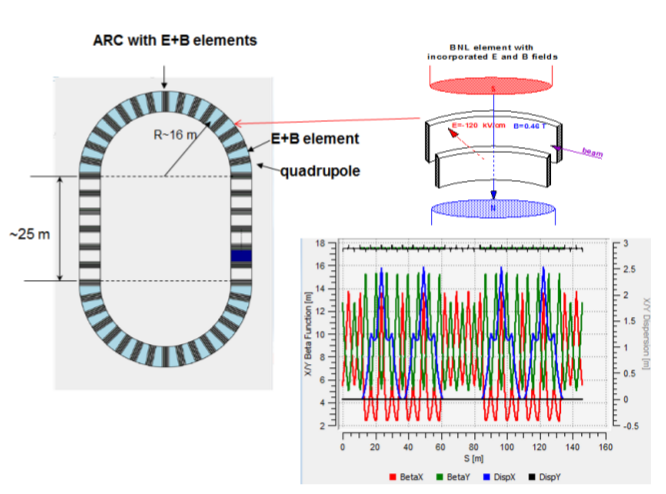
\includegraphics[width=\linewidth]{images/chapter2/BNL_lattice}
	\caption{A FS lattice variant. Cylindrical E+B spin-rotators are used in the arc sections to fulfill
          the FS condition. (Image is taken from~\cite{Senichev:Lattices}.)\label{fig:BNL_lattice}}
\end{figure}

The main purpose of a FS lattice is to maximize the EDM signature signal. However, it is important to note that,
strictly speaking, the FS condition is held only the reference particle. This is because, as follows from
equation~\eqref{eq:TBMT_MDM}, for any given E- and B-fields there exists a unique value of the Lorentz factor
$\gamma$ at which $\W_y^{MDM} = 0$. Hence, even in a FS lattice, most particles' spin vectors are frozen only
approximately.

\subsection{Quasi-Frozen Spin lattice} \label{chpt2:concept:QFS}
In the QFS design concept, one gives up the continuity property of the FS condition, requiring only that the spin
phase advance (in the rest frame) in the electrostatic ($\Phi_s^E$) and magnetic ($\Phi_s^B$) elements was zero
on average (turn by turn):~\cite{Senichev:Lattices}
\begin{equation*}
	\sum_i \Phi_{s,i}^E = -\sum_j \Phi_{s,j}^B.
\end{equation*}

Following the definition of spin tune (see section~\ref{sec:TBMT_introduction}), a particle's spin vector
placed into an electromagnetic field turns by angle $\Phi_s = \nu_s \cdot \Phi$, where $\Phi$ is
the momentum rotation angle, $\nu_s$ spin tune.

A particle's angular momentum, when placed into a magnetic field $\vec B$ is
\[
\w_B = \frac qm \frac B \gamma,
\]
into an electrostatic $\vec E$:
\[
\w_E = \frac qE \frac{\vec E\times \vec\beta}{c\beta^2\gamma},
\]
from which follow the expressions for spin tune in the electrostatic and magnetic fields:
\begin{equation}
	\begin{cases}
		\nu_s^B &= \gamma G, \\
		\nu_s^E &= \beta^2\gamma\bkt{\frac{1}{\gamma^2-1} - G}.
	\end{cases}
\end{equation}

The QFS lattice design has the advantage of simplicity over the FS one: there's no need to use a combined-field
cylindrical spin rotators; in both QFS lattice variants we consider below are used either
\begin{enumerate*}[\itshape a\upshape)]
\item straignht Wien filters,  or
\item cylindrical electrostatic and magnetic elements separately.
\end{enumerate*}
On the other hand, due to the appearance of a vertical spin precession axis component $\bar n_y$,
the maximum EDM signal amplitude is less compared with the pure FS case. Teh attenuation
factor~\cite{Senichev:QFS_IPAC15}
\[
J_0(\Phi_s) \approx 1 - \frac{\Phi_s^2}{4},
\]
where $\Phi_s$ is the maximum horizontal plane spin phase advance. Assume the phase advance does not
exceed $\pi\cdot \gamma G/2n$; in this context $n$ is the lattice periodicity. Since the deuterin animalous magnetic moment $G = -0.142$, for the QFS lattices considered below $J_0\ge 0.98$.

\subsubsection{QFS lattice design ``6.3''}\label{chpt2:lattice:QFS:6_3}

In Figure~\ref{fig:QFS_6_3_lattice} is presented a QFS design lattice in which the E- and B-fields are
separated in space.~\cite{Senichev:Lattices} Negative radius electrostatic cylindrical deflectors are used
to compensate the spin phase advance related to the MDM precession in the arc sections.~\cite{Senichev:QFS_IPAC15}
The ring is 166.67~m length long and is dessigned for the 270 MeV injection energy. For the suppression
of linear spin decoherence effects, an RF cavity is used, with voltage $V = 100$ kV, and operating
frequency $f_{RF} = 5\cdot f_{rev}$, where $f_{rev} = 0.87$ MHz. Non-linear decoherence effects are suppressed
by using six sextupole families.

\begin{figure}[h!]
	\centering
	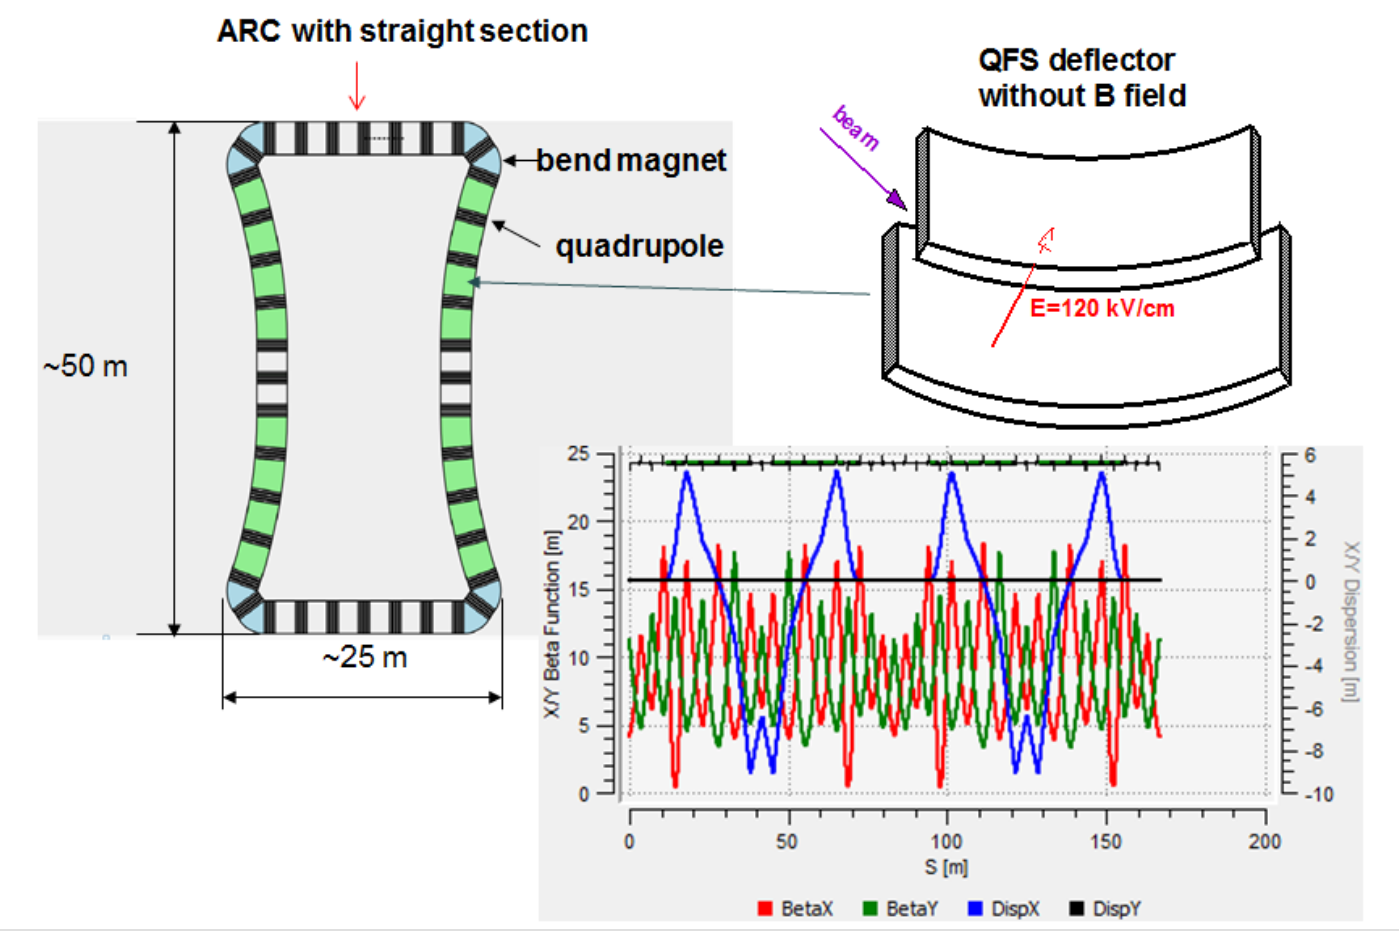
\includegraphics[width=\linewidth]{images/chapter2/6_3_lattice}
	\caption{QFS lattice design variant with spatially separated E- and B-fields.
          (Image taken from~\cite{Senichev:Lattices})\label{fig:QFS_6_3_lattice}}
\end{figure}

\subsubsection{QFS lattice design ``E+B''}\label{chpt2:lattice:QFS:EB}

The lattice design in Figure~\ref{fig:QFS_E+B_lattice} uses plain straight, static Wien filters.
This allows one to:
\begin{enumerate*}[\itshape a\upshape)]
	\item exclude non-linear electrostatic field components present in curved electrostatic fields, and 
	\item simplify the lattice from the engineering point of view.
\end{enumerate*}

The lattice is 149.21~m in length, the injection energy is 270 MeV. The linear spin decoherence effets suppressing
RF cavity has a longitudinal voltage $V = 100$ kV, and frequency $f_{RF} = 5\cdot f_{rev}$,
with $f_{rev} = 0.98$ MHz. Four sextupole families are used for the suppression of non-linear decoherence effects.
\begin{figure}[h!]
	\centering
	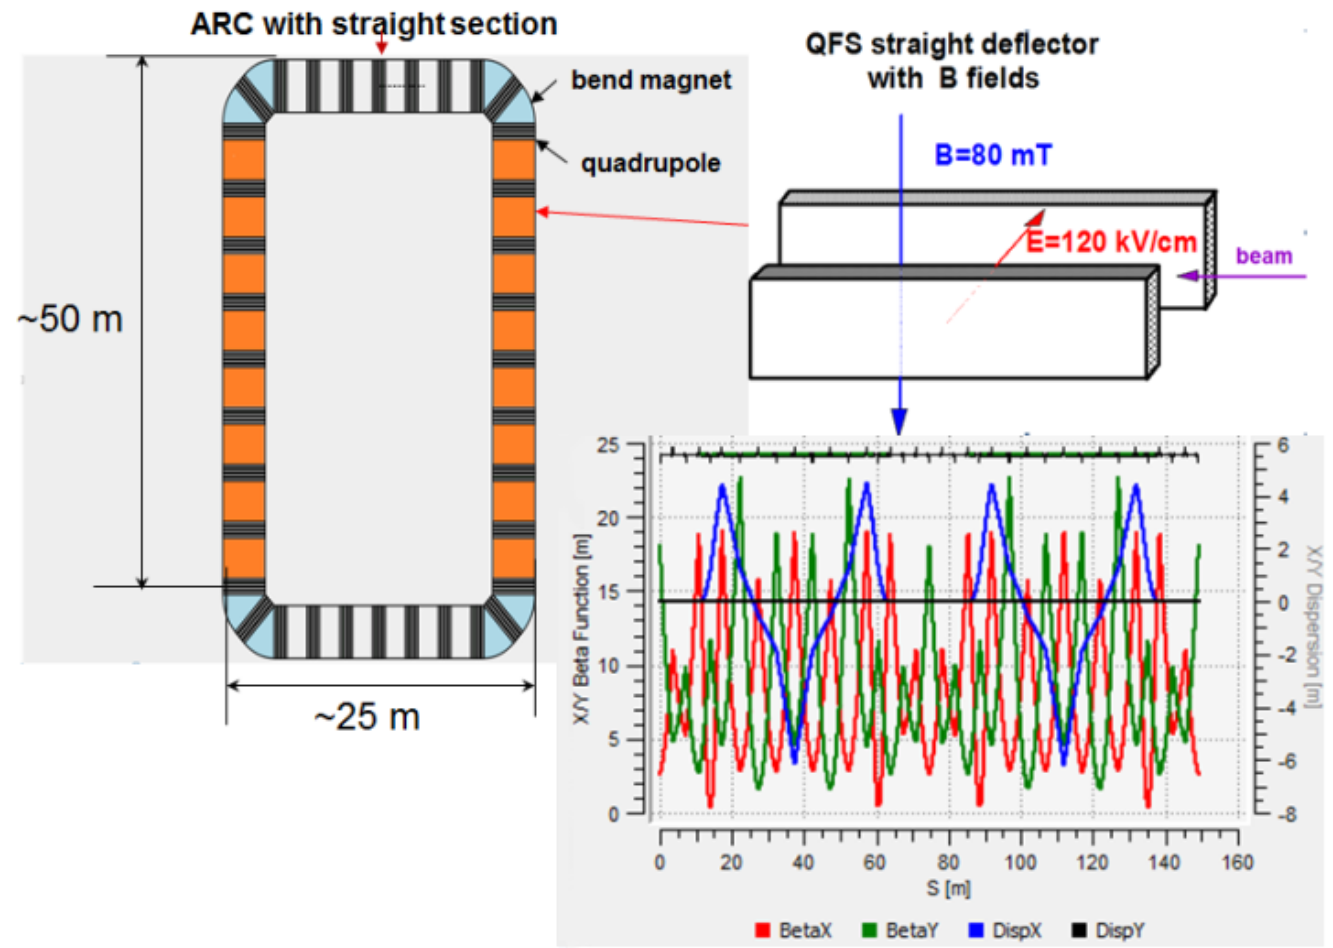
\includegraphics[width=\linewidth]{images/chapter2/E+B_lattice}
	\caption{Straight Wien filters QFS lattice variant.
          (Image taken from~\cite{Senichev:Lattices})\label{fig:QFS_E+B_lattice}}
\end{figure}



\clearpage
